% ==================================================================
\section{Recursive: Tree Task Decomposition}
\label{sec:rec-tree}
% ==================================================================

\subsection{Implementation}
\label{sec:rec-tree-impl}
El codi de la versió \textbf{tree recursive} es troba a \texttt{mandel-omp-tree.c}.\\
En aquest cas, com a la versió \textbf{leaf}, la regió paral·lela es crea al main, abans de la crida a \texttt{mandel\_tiled\_rec}, declarant la regió com a \texttt{single}. Inicialment, un únic thread inicia el recorregut recursiu, però a diferència de l'estratègia \textbf{leaf}, es creen tasques per a totes les crides recursives, no només per a les fulles de l'arbre de recursió. Això permet que, des de ben aviat, múltiples threads puguin agafar tasques i generar-ne de noves en paral·lel, distribuint així la creació de tasques entre tots els threads disponibles.\\
Veguem ara com es creen les tasques. En primer lloc, i en diferència a la versió \textbf{leaf}, es pararel·litza la comprovació de si les boreres del tile són iguals:
\begin{lstlisting}[caption={Creació de tasques per a la comprovació de les boreres.},label={lst:rec-tree-tasks}]
    int equal,equalH,equalV;
    equal = non_first_call;
	equalH = non_first_call;
	equalV = non_first_call;
	#pragma omp taskgroup
	{
	#pragma omp task shared(equalH)
	{

      for (int py = y; py < y + NRows; py++) {
	    M[py][x] = pixel_dwell(COLS, ROWS, CminR, CminI, CmaxR, CmaxI, x, py, scale_real, scale_imag, maxiter);
	    M[py][x + NCols - 1] = pixel_dwell(COLS, ROWS, CminR, CminI, CmaxR, CmaxI, x + NCols - 1, py, scale_real, scale_imag, maxiter);
	    equalH = equalH & (M[y][x] == M[py][x]);
	    equalH = equalH & (M[y][x] == M[py][x + NCols - 1]);
      }
	}

	#pragma omp task shared(equalV)
	{
	
      for (int px = x; px < x + NCols; px++) {
	    M[y][px] = pixel_dwell(COLS, ROWS, CminR, CminI, CmaxR, CmaxI, px, y, scale_real, scale_imag, maxiter);
	    M[y + NRows - 1][px] = pixel_dwell(COLS, ROWS, CminR, CminI, CmaxR, CmaxI, px, y + NRows - 1, scale_real, scale_imag, maxiter);
	    equalV = equalV & (M[y][x] == M[y][px]);
	    equalV = equalV & (M[y][x] == M[y + NRows - 1][px]);
      }
	}

	}
	equal = equalH & equalV;
\end{lstlisting}

A diferència de la versió \textbf{leaf}, aquí la creació de tasques no és sequencial, sinó que es poden crear tasques per a la comprovació de les boreres en paral·lel. Això permet que, des de ben aviat, múltiples threads puguin agafar tasques i generar-ne de noves en paral·lel, distribuint així la creació de tasques entre tots els threads disponibles. Augmentem així els fragments de codi que podem executar en paral·lel. Creem un taskgroup per assegurar que la comprovació equal = equalH \& equalV es fa un cop s'han executat les tasques, i fem les variables shared, permetent així la consulta i la concordància del valor a fora de la tasca.\\
Posteriorment, es creen tasques per a les crides recursives, de manera que la creació de tasques es distribueix entre tots els threads disponibles. Veiem la regió de codi:\\
\begin{lstlisting}[caption={Creació de tasques per a les crides recursives.},label={lst:rec-tree-tasks2}]
    else {
		  if (NRows > TILE) {
			#pragma omp task
			{
			mandel_tiled_rec(M, NRows / 2, NCols / 2, start_fil, start_col, CminR, CminI, CmaxR, CmaxI, scale_real, scale_imag, maxiter);
			}
			#pragma omp task
			{
			mandel_tiled_rec(M, NRows / 2, NCols / 2, start_fil + NRows / 2, start_col, CminR, CminI, CmaxR, CmaxI, scale_real, scale_imag, maxiter);
			}
			#pragma omp task
			{
			mandel_tiled_rec(M, NRows / 2, NCols / 2, start_fil, start_col + NCols / 2, CminR, CminI, CmaxR, CmaxI, scale_real, scale_imag, maxiter);
			}
			#pragma omp task
			{
			mandel_tiled_rec(M, NRows / 2, NCols / 2, start_fil + NRows / 2, start_col + NCols / 2, CminR, CminI, CmaxR, CmaxI, scale_real, scale_imag, maxiter);
			}

		  } else {
			#pragma omp task
			{
			mandel_tiled_rec(M, NRows, NCols / 2, start_fil, start_col, CminR, CminI, CmaxR, CmaxI, scale_real, scale_imag, maxiter);
			}
			#pragma omp task
			{
			mandel_tiled_rec(M, NRows, NCols / 2, start_fil, start_col + NCols / 2, CminR, CminI, CmaxR, CmaxI, scale_real, scale_imag, maxiter);
			}

		  }

	    }
\end{lstlisting}
Cal destacar també que s'han evitat els problemes de data sharing de la mateixa manera que en l'estratègia \textbf{leaf}.

\paragraph{Comparació amb Improved Leaf.}

\subsection{Modelfactor Analysis}
\label{sec:rec-tree-mf}

\begin{figure}[H]
    \centering
    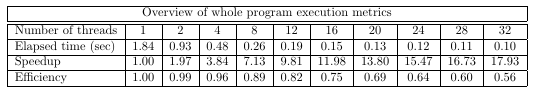
\includegraphics[width=0.9\linewidth]{fotosL4/primera_tabla_tree.png}
    \caption{Model factor 1 (Tree).}
    \label{fig:rec-tree-mf1}
\end{figure}

\begin{figure}[H]
    \centering
    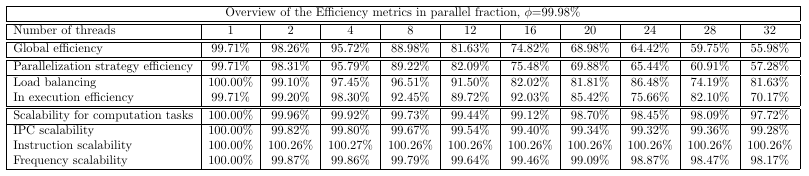
\includegraphics[width=0.9\linewidth]{fotosL4/segunda_tabla_tree.png}
    \caption{Model factor 2 (Tree).}
    \label{fig:rec-tree-mf2}
\end{figure}

\begin{figure}[H]
    \centering
    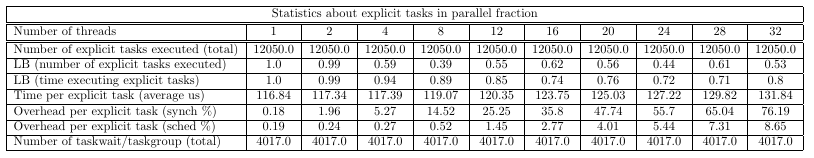
\includegraphics[width=0.9\linewidth]{fotosL4/tercera_tabla_tree.png}
    \caption{Model factor 3 (Tree).}
    \label{fig:rec-tree-mf3}
\end{figure}
A la primera taula destaca la millora en els resultats respecte les estratègies leaf. Veiem com l'Elapsed Time es redueix significativament, gairebé a la meitat els primers cops que dupliquem el nombre de threads, i que es redueix fins als 32 threads arrribant a un valor de 0.10 s, tot i així, a partir dels 16, la dismunució ja no és tan notoria.\\
Notem també que el SpeedUp millora molt sempre que augmentem el nombre de threads, son bons resultats, arribant a un Speedup de 17.93 amb 32 threads. Destaca també que l'Efficiency es manté força alta, major al 80\% fins als 12 threads i que en qualsevol cas, no baixa del 50\% en els casos estudiats.\\
Veiem a la segona taula que els valors de Load Balancing són molt millors que a la versió leaf, superiors al 90\% fins als 12 threads i després encara superiors al 80\%, cosa que indica que els threads estan molt ben equilibrats, i això es deu a què la creació de tasques es distribueix entre tots els threads disponibles.\\
Finalment, a la tercera taula destaca que el nombre de tasques executades és de 12015, molt superior al nombre de tasques executades a la versió leaf (gairebé quadriplicant), que era de 3013, i això es deu a què en aquesta versió es creen tasques per a totes les crides recursives, no només per a les fulles de l'arbre de recursió.\\

\subsection{Paraver Analysis}
\label{sec:rec-tree-paraver}

% Paraver trace (task creation / useful parallelism)
\begin{figure}[H]
    \centering
    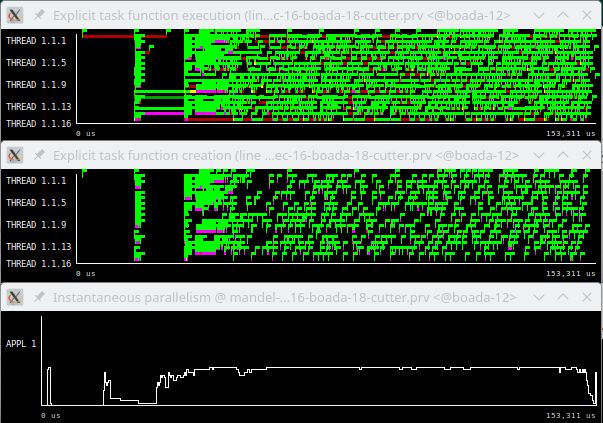
\includegraphics[width=0.9\linewidth]{fotosL4/paraver_tree.png}
    \caption{Paraver trace for Recursive Tree (16 threads): task density and execution.}
    \label{fig:rec-tree-paraver}
\end{figure}

A les traces obtingudes amb Paraver, podem observar el següent: d'una banda, veiem com tots els threads creen i executen tasques, a diferència de la versió leaf. Destaca també com inicialment, només un thread crea la tasca, hi ha un periode d'execució, en que no es creen ni s'executen tasques, i després, a mesura que es creen tasques, més threads s'incorporen a l'execució, i es van creant i executant tasques en paral·lel. Això es veu reflectit també en la densitat de tasques.
Veiem també, en relació a com s'inicia la creació de tasques, que a la traça inferior s'observa d'inici que es creen valls de threads actius, això es correspon amb el fet de que fins que no s'assoleix una certa profunditat en la recursió, no hi ha suficients tasques com per mantenir ocupats a tots els threads, però a mesura que es creen més tasques, més threads s'incorporen a l'execució. Destaca, en contrast amb l'estratègia leaf, que en el general de l'execució, l'ocupació dels threads roman molt més alta i estable.

\subsection{Strong Scalability}
\label{sec:rec-tree-scalability}

% Strong scalability plot
\begin{figure}[H]
    \centering
    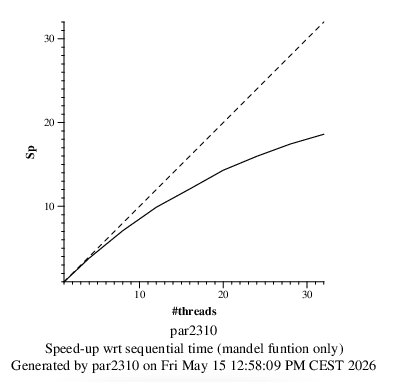
\includegraphics[width=0.75\linewidth]{fotosL4/grafico_tree.png}
    \caption{Strong scalability (elapsed time vs. threads) for the Recursive Tree implementation.}
    \label{fig:rec-tree-speedup}
\end{figure}
S'observa a la figura, tot i que ja s'ha esmentat, com l'SpeedUp millora molt en els primers increments del numero de threads, gairebé al ritme de la linia discontinua, però que a mesura que s'augmenta deixa d'augmentar tant notoriament l'SpeedUp.
Això s'analitza com que arriba un punt on afegir més threads no aporta tanta millora, ja que el nombre de tasques disponibles per executar no és suficient com per mantenir a tots ocupats, afegint a més més necesitat de sincronització entre threads.